%    Author: David Riser, University of Connecticut 
%    File: thesis/chapters/sidis.tex
%
%    Change Log:
%    ----------- 
%    - 2018/09/18: Splitting inclusive cross section information
%                  out of this document and adding it to another 
%                  document chapters/inclusive.tex.  
%
%    Random Thought: 
%    ---------------
%    This chapter describes the work done primarily by Nathan Harrison
%    in his construction of the observables listed below for both charged
%    pions.  In writing these sections, I need to strike a delicate balance
%    between attributing the credit to him, and depicting that I did 
%    contribute a significant amount of work to the study.  
%
%
%
%    Chapter Structure:
%    -------------------
%    - Statement of purpose and overview of chapter.
%    - Introduction, necessary theory to understand the results presented.
%    - Hadronic identification, different for this study than described in the particle identification chapter.
%    - Event Selection (DIS cuts, missing mass cuts, y cut)
%    - Binning 
%    - Data distributions
%    - MC simulation details and generated/reconstructed distributions
%    - Acceptance corrections, iterative procedure description
%    - Radiative corrections (how did this occur, read Nathan's thesis)
%    - Systematic uncertainties
%    - Results 
 

\chapter{SIDIS Cross Section}
This chapter discusses the analysis of semi-inclusive deeply inelastic events.  After a brief motivation, the data analysis details are described.  

\section{Introduction}
The primary goal of this work is to provide the SIDIS cross section for charged pions ($\pi^{\pm}$) over a large kinematic range ($0.1 < x < 0.6$, $1.0 < Q^2 < 4.7$, $0.0 < z < 0.9$, $0.0 < P_{T}^{2} < 1.0$, $-180^\circ < \phi_h < 180^\circ$).  Fortunately these channels were studied by Nathan Harrison and the CLAS collaboration \cite{theses-harrison:2015} using the E1-F dataset (2010-2015).  By writing the cross section as, 

\begin{equation}
	\frac{d^5\sigma}{dx \; dQ^2 \; dz \; dP_T^2 \; d\phi_h} = A_{0} \Bigl[ 1 + A_{UU}^{\cos\phi_h} \cos\phi_h + A_{UU}^{\cos(2\phi_h)} \cos(2\phi_h) \Bigr]
\end{equation}

Harrison et al. measured the un-normalized quantities $A_0$, $A_{UU}^{\cos\phi}$, and $A_{UU}^{\cos(2\phi)}$ which are defined below.  

\begin{gather}
	A_{0} = \frac{\pi \alpha^2 y (1+\gamma^2/2x)}{2 E M_p x^2 Q^2 (1-\varepsilon)} \Bigl( F_{UU,T} + \varepsilon F_{UU,L} \Bigr) \\
	A_{UU}^{\cos\phi_h} = \sqrt{2\varepsilon(1+\varepsilon)} \frac{F_{UU}^{\cos\phi_h}}{F_{UU,T} + \varepsilon F_{UU,L}} \\
	A_{UU}^{\cos(2\phi_h)} = \varepsilon \frac{F_{UU}^{\cos(2\phi_h)}}{F_{UU,T} + \varepsilon F_{UU,L}}
\end{gather}

In order to measure the structure functions $F_{UU}^{\cos\phi_h}$ and $F_{UU}^{\cos(2\phi_h)}$ directly, the integrated luminosity is needed.  The calculation of this quanitity for E1-F is described in detail during chapter 2 of this document.  Experimentally, the cross section in the $i^{th}$ bin is given as, 

\begin{equation}
	\frac{d\sigma}{dx \; dQ^2 \; dz \; dP_T^2 \; d\phi_h} = \frac{1}{\Delta x \; \Delta Q^2 \; \Delta z \; \Delta P_T^2 \; \Delta \phi_h} \frac{N_{obs}^{(i)}}{\mathcal{L} A^{(i)} R^{(i)}} 
\end{equation}

where the superscript $(i)$ reminds the reader that these quantities are calculated for every bin.  Throughout this chapter the symbols $A^{(i)}$, $R^{(i)}$, and $B^{(i)}$ refer to the acceptance correction, radiative correction, and bin centering correction respectively.  These factors will be described in more details in this chapter. Finally, the $\Delta$ factors here denote the width of each bin in 1 dimension of the 5-dimensional space (non-uniform sized bins may be used, in which case this factor also carries an index $(i)$).\\

The integrated luminosity obtained in chapter 2 can be directly applied to the measurement of Harrison et al. to produce 5-dimensional differential cross sections.  This procedure is carried out, but only after the luminosity factor is independently verified by calculating the cross section for inclusive inelastic electron scattering in the resonance region (here $1.1 < W < 2.1 \; GeV/c^2$).  Accurate models for the inclusive cross section exist based on phenomenological fits to existing datasets.  For verification, we compare the cross section from E1-F to a model created by Cynthia Keppel \cite{find-keppel-reference}. \\

The calculation of the inelastic scattering cross section as described here is non-trivial, and (together with the phenomenological analysis presented in chapter 6) constitutes the main original effort expent by the authors.    

\section{Hadron Identification}
%
% The hadron ID isn't the same as mine from chapter 4 because we're extending Nathan's work.
%

As was described in chapter 4, the classification of hadrons in CLAS is done by using the momentum measurement as well as the time of flight measurement.  By using the electron to calculate a start time and the distance along the fit hadron candidate track to the time of flight paddle, the velocity fraction $\beta = v/c$ is calculated for candidates.  Hadrons with mass $m$ and momentum $p$ are theoretically expected to have a $\beta_{exp}$ value given in equation \ref{equation:betap}.  This equation has the important feature that for a fixed momentum value, hadrons with different masses are separated in their $\beta$ values.

\begin{equation}
	\label{equation:betap}
	\beta_{exp} (p) = \frac{1}{\sqrt{1 + (m/p)^2}}
\end{equation}

In chapter 4, the hadronic identification methods described used a probabilistic interpretation of the difference between the observed values of $\beta$ and the expected values given by \ref{equation:betap} (or determined by fitting small deviations from the theoretical case).  This study was performed before that identification routine was developed, and therefore uses a slightly different boundary and interpretation (described first by N. Harrison in his thesis work \cite{theses-harrison:2015}).  Fiducial cuts used for positives and negatives are exactly identical to those described in chapter 4, and will not be discussed here.  \\

In order to determine the cut boundaries, the events are fit in each of 70 momentum bins and the mean $\mu$ and standard deviation $\sigma$ are recorded.  Pions which fall between $\mu - 3\sigma \leq \beta \leq \mu + 3 \sigma$ are kept for analysis.  At higher momentum positive pi-mesons are difficult to separate from protons than at lower momentum values.  To accommodate this, the $\sigma$ value is reduced after 2 GeV.  \\

\begin{table}
	\label{table:hadron-id-nathan}
  \centering
  \begin{tabular}{c|c|c}
    Hadron & $p_{min}$ (GeV) & $p_{max}$ (GeV) \\
    \hline 
	\pi^+ & 0.2 & 3.75 \\
	\pi^- & 0.2 & 3.25 \\
  \end{tabular}
  \caption[Limits for pion momentum used in fitting $\beta$.]{The limits used for pion momentum used in the fitting of $\beta$ for both charged pi-mesons.}
\end{table} 
 
\section{Event Selection}
The identification of an event which contains a good electron and a good pion ($\pi^{\pm}$) is the first step in selecting SIDIS events from the dataset.  Next, events that meet the working assumption for what constitutes the DIS region are selected by calculating the electron kinematics of the event and requiring that the negative momentum transfer squared $Q^2 > 1.0 \; GeV^2$ and $W > 2.0 \; GeV$.  Formally the SIDIS process includes a sum over all possible final states. However, a missing mass cut is used in this analysis to remove low lying exclusive resonances which are not dominantly produced by the SIDIS mechanism.  Accordingly it is required that the missing mass $M_X (e p \rightarrow)e h X$ be greater than 1.35 GeV (in the positive channel this excludes the delta resonance).  \\

One additional kinematic restriction is applied at the event selection stage, a cut on the maximum allowable inelasticity $y_{max}$.  Full radiative corrections will be discussed in detail, but this kinematic restriction excludes events which have extremely high values of $Q^2$ and are much more likely to have radiated a photon in the initial or final state.  In this analysis $y_{max} = 0.85$ is used.  

\section{Binning}
Both $\pi^+$ and $\pi^-$ are binned using the same scheme.  The momentum fraction $x$ is divided into five equally sized bins from 0.1 - 0.6, each of which is split into two $Q^2$ low/high bins, with the exception of the highest $x$ bin, which only contains one $Q^2$ bin.  This binning scheme for $x-Q^2$ is displayed in figure \ref{fig:kinematics-xq2}.  \\

\begin{figure}
  \centering
  \label{fig:kinematics-xq2}
  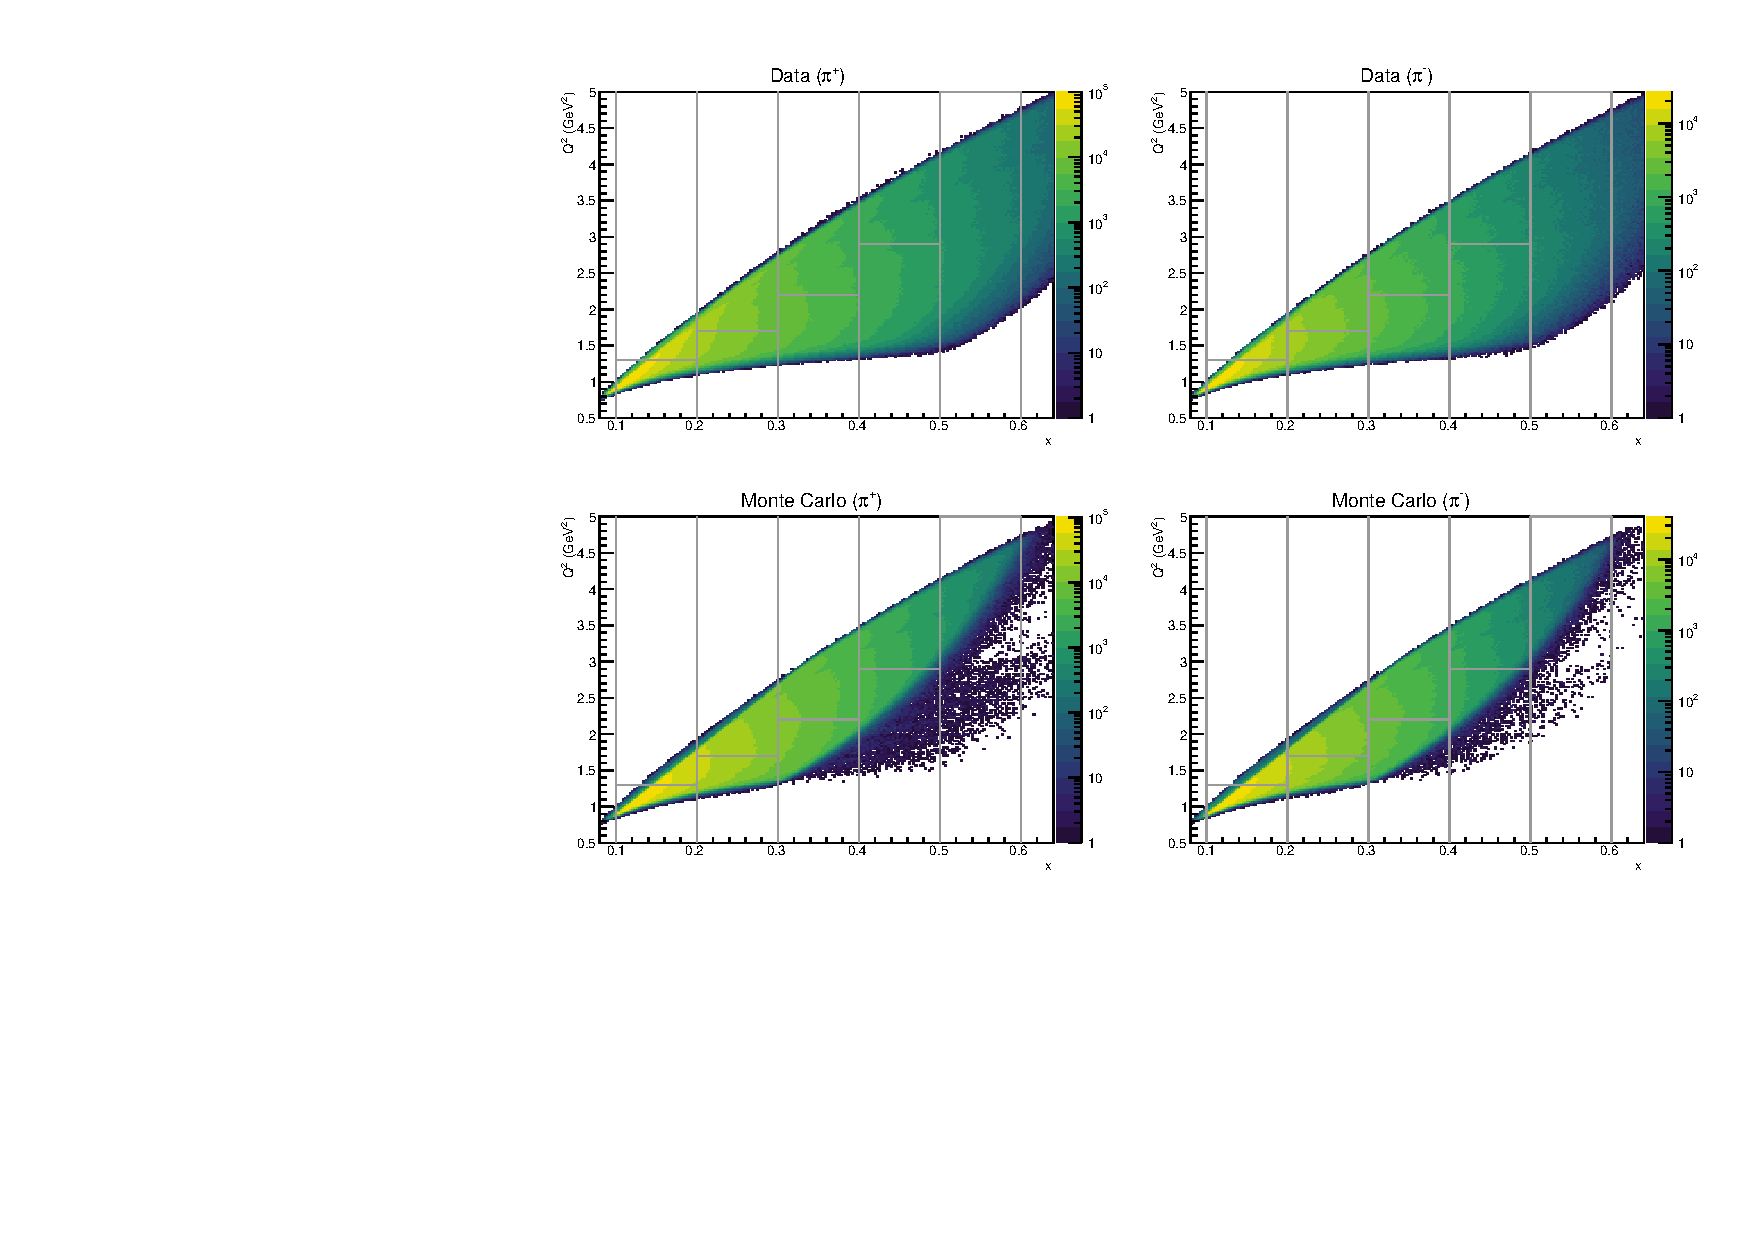
\includegraphics[width=\textwidth]{image/plots/sidis/xq2.pdf}
  \caption[Kinematic distributions and binning for electron variables.]{The kinematic distributions for $\pi^{\pm}$ electron variables shown with binning overlaid.}
\end{figure}
\begin{figure}
  \centering
  \label{fig:kinematics-zpt}
  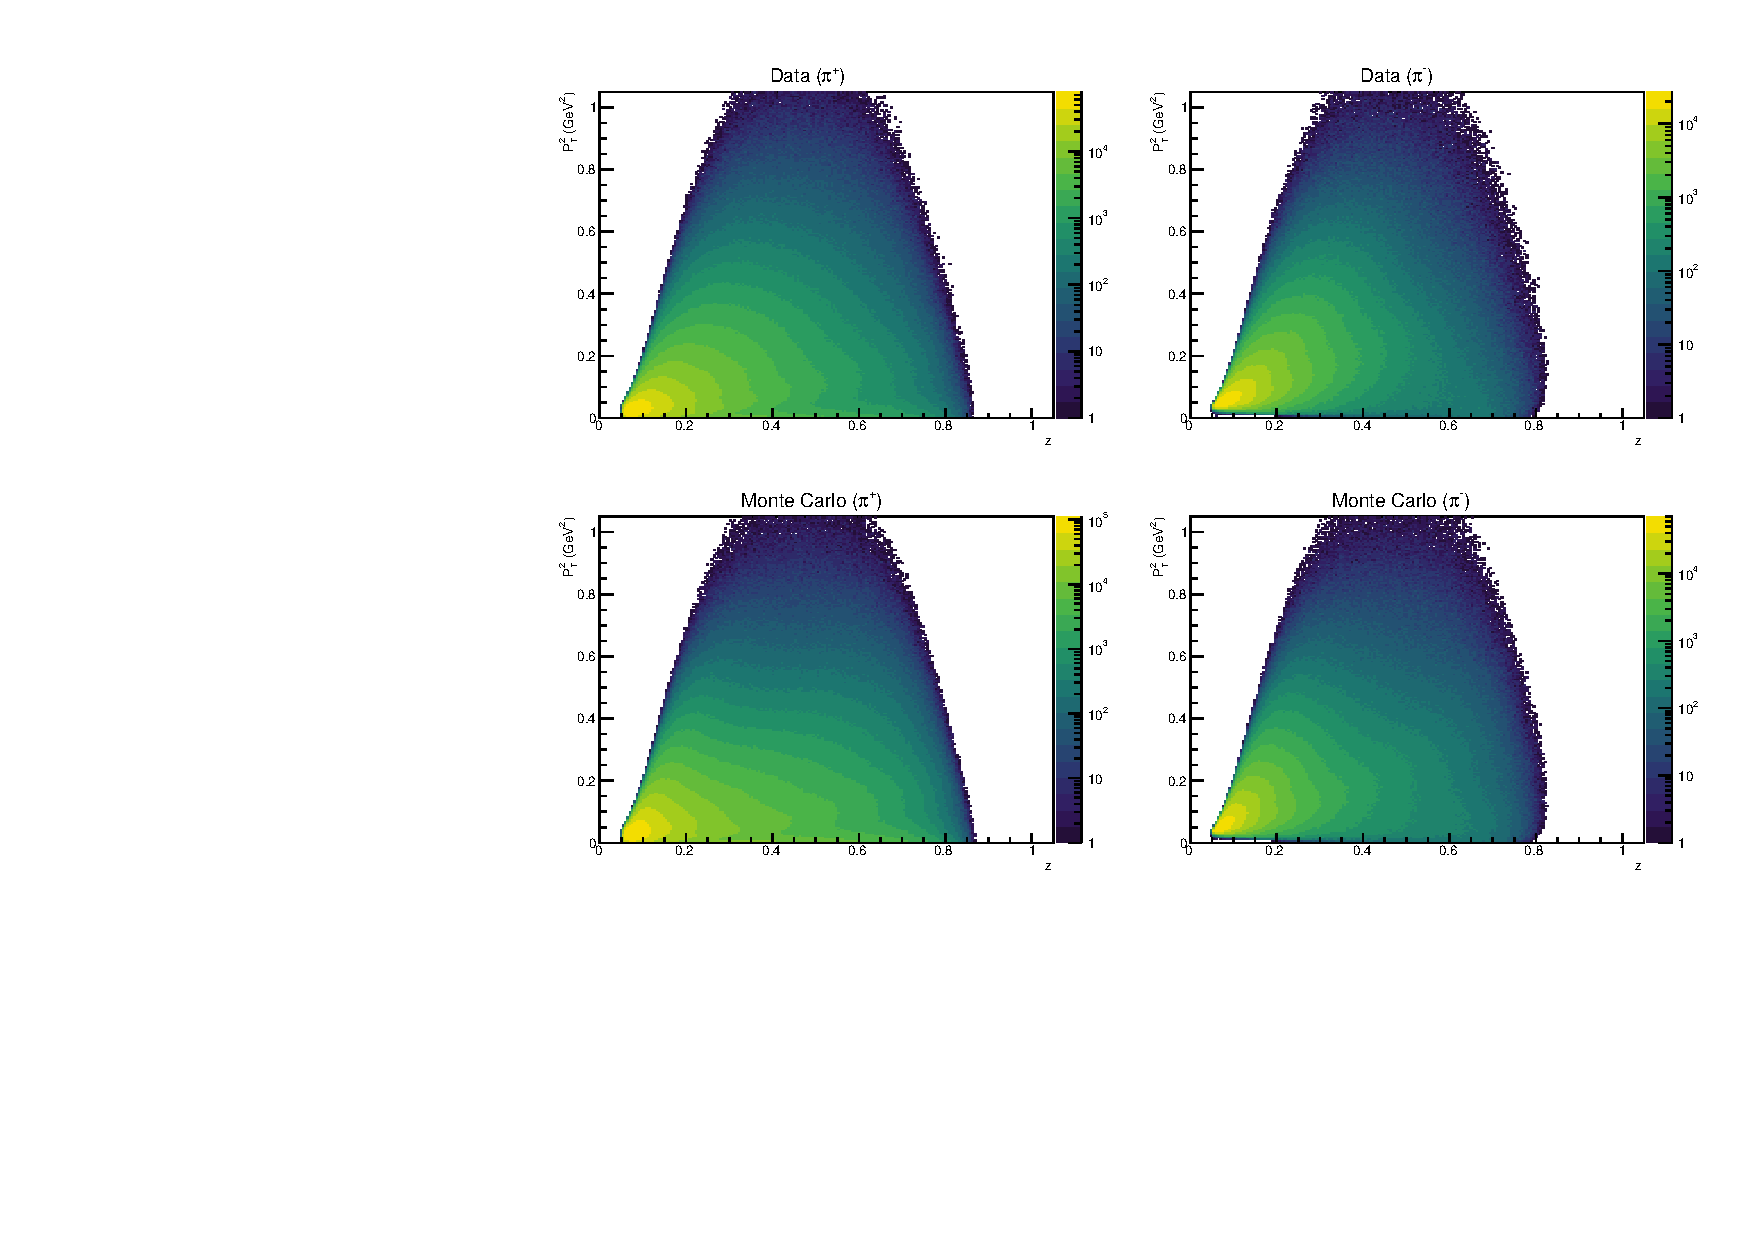
\includegraphics[width=\textwidth]{image/plots/sidis/zpt.pdf}
  \caption[Kinematic distributions and binning for hadron variables.]{The kinematic distributions for $\pi^{\pm}$ hadron variables shown with binning overlaid.}
\end{figure}

The hadronic variables are binned finer, the $z$ axis is divided into 18 equal sized bins between 0-0.9, and the transverse momentum squared $P_T^2$ is binned in 20 equally sized bins from 0-1 $GeV^2$.  This simple grid is shown on figure \ref{fig:kinematics-zpt}.

\section{MC Simulation}
Show rec/gen distributions and discuss the event generator used in this study.

\section{Acceptance Corrections}

\begin{sidewaysfigure}
  \centering
  \label{fig:acceptance}
  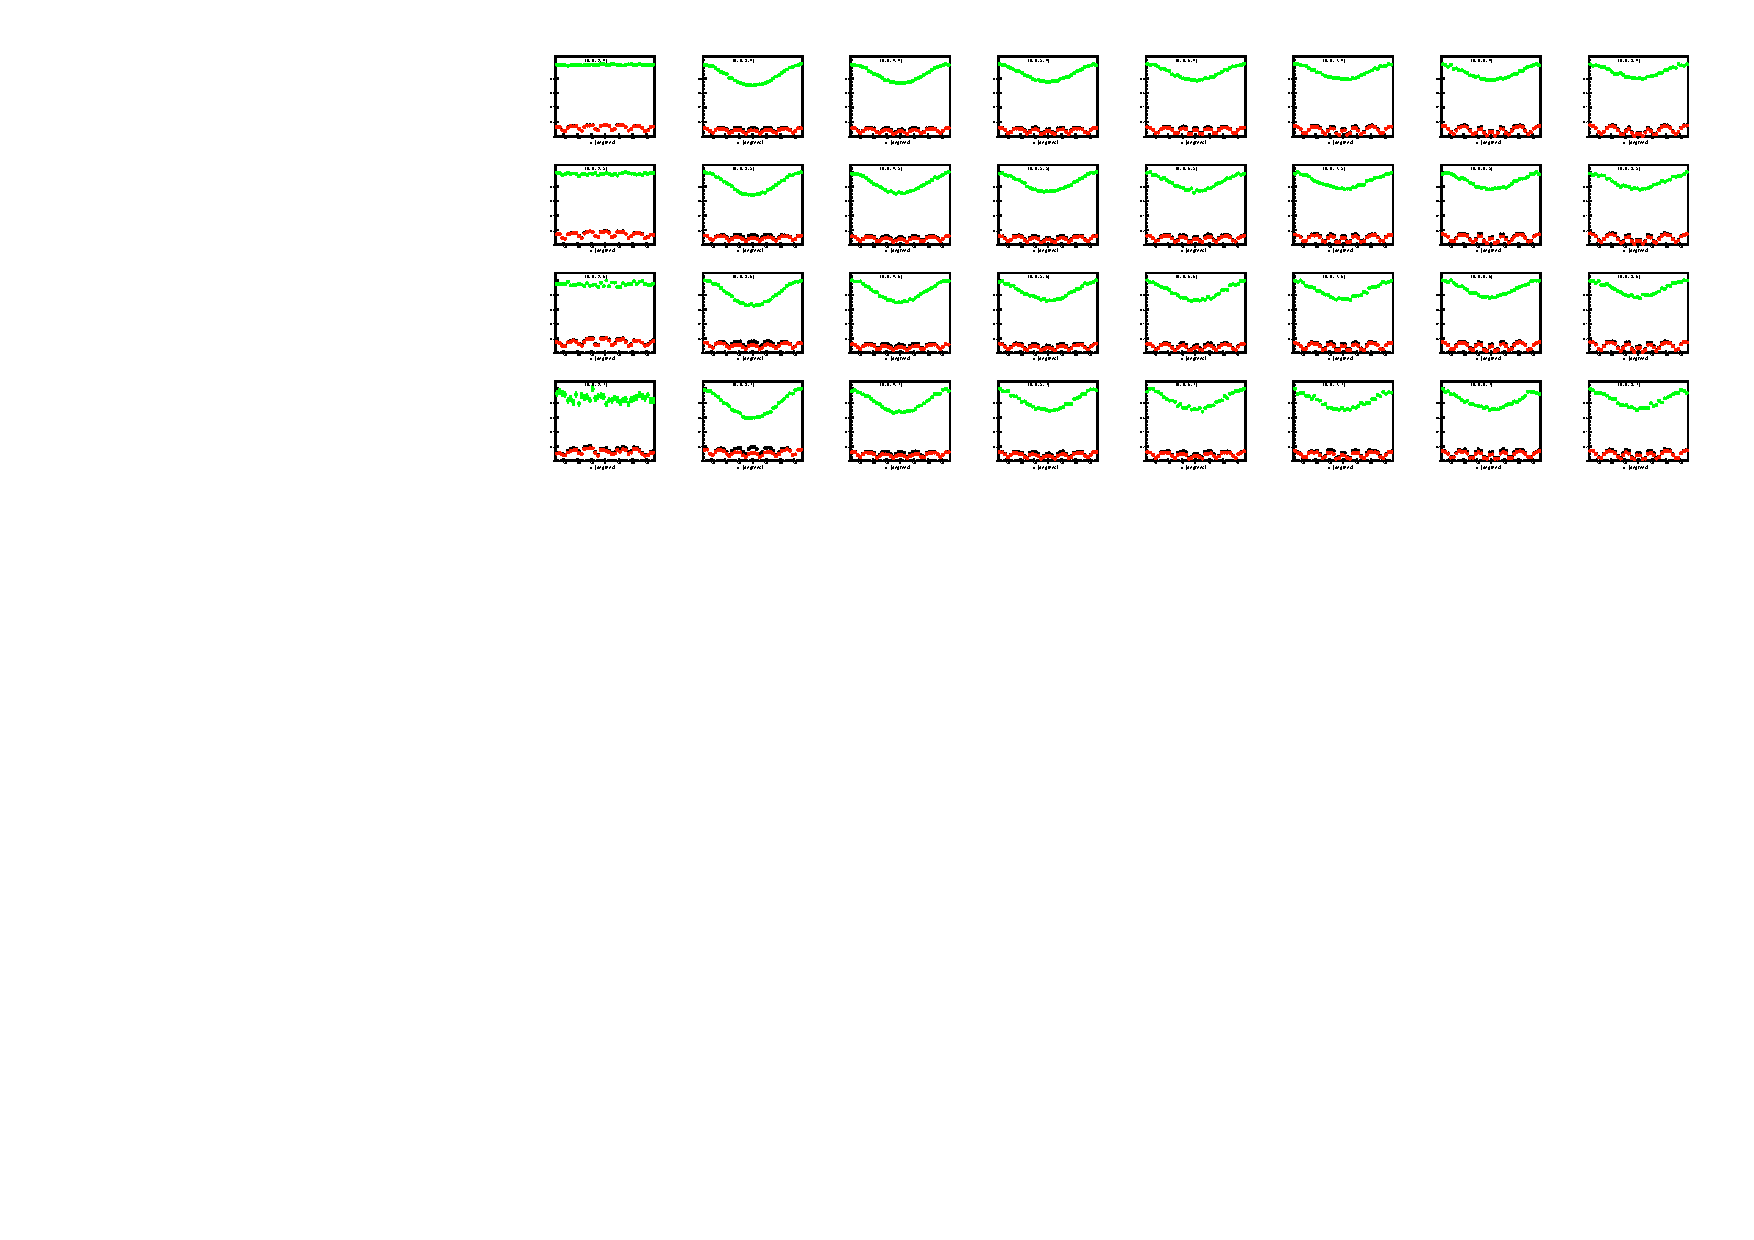
\includegraphics[width=\textwidth]{image/plots/sidis/acceptance.pdf}
  \caption[Acceptance corrections for SIDIS]{Acceptance corrections shown for different $z$ bins (increasing over the horizontal axis) and $P_{T}^{2}$ bins (increasing down the vertical axis) are displayed in red.  Generated events are displayed in green, and in red the reconstructed events are shown normalized by the maximum number of generated events in any bin.  On each figure the complete bin index is given in the format $(x, Q^2, z, P_{T}^{2})$.}
\end{sidewaysfigure}

\section{Radiative Corrections}
Here we discuss HAPRAD.

\section{Systematic Uncertainties}

\begin{sidewaysfigure}
  \centering
  \label{fig:systematics-region1}
  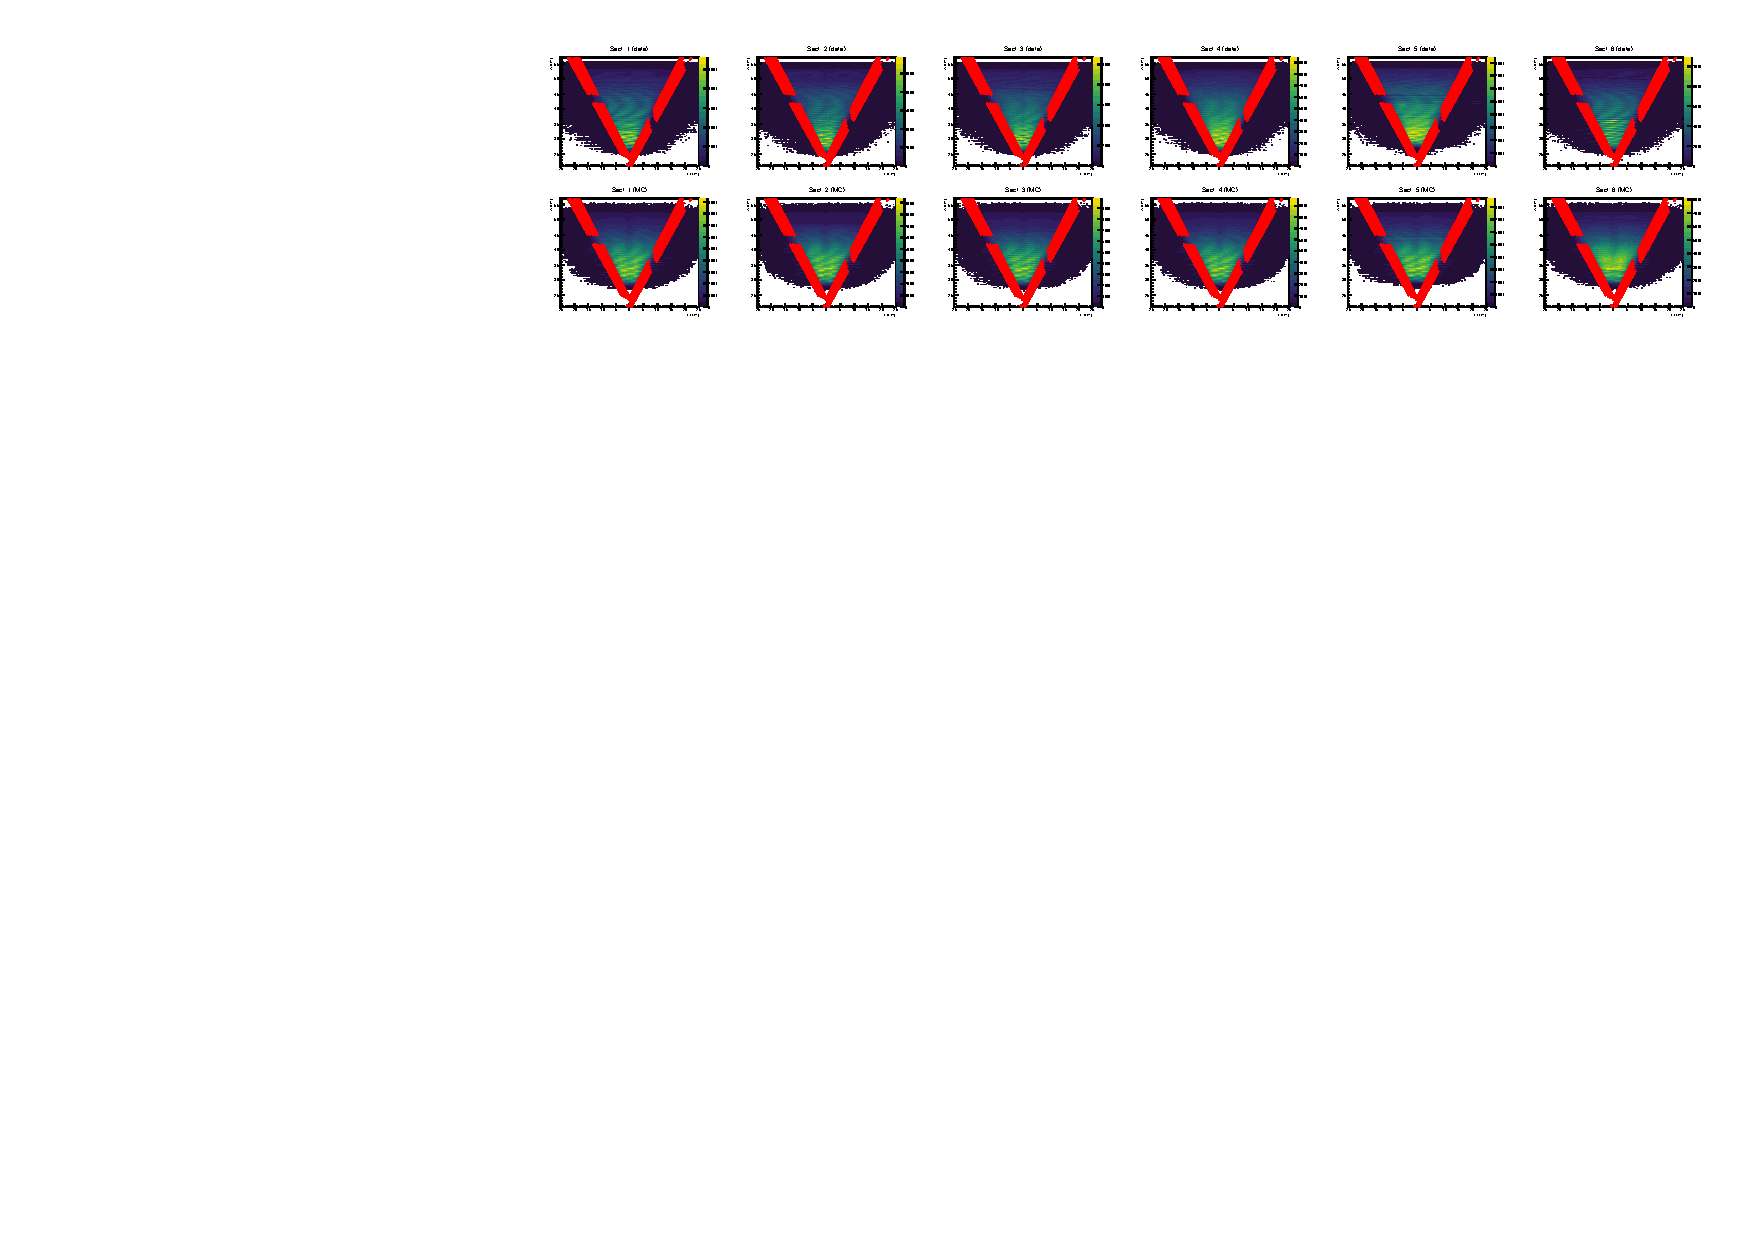
\includegraphics[width=\textwidth]{image/plots/sidis/systematics/region1.pdf}
  \caption[Systematic boundaries on region 1]{Boundaries for electron identification cuts placed on the region 1 drift chambers are shown for data (top row) and Monte Carlo (bottom row).}
\end{sidewaysfigure}

\begin{sidewaysfigure}
  \centering
  \label{fig:systematics-region3}
  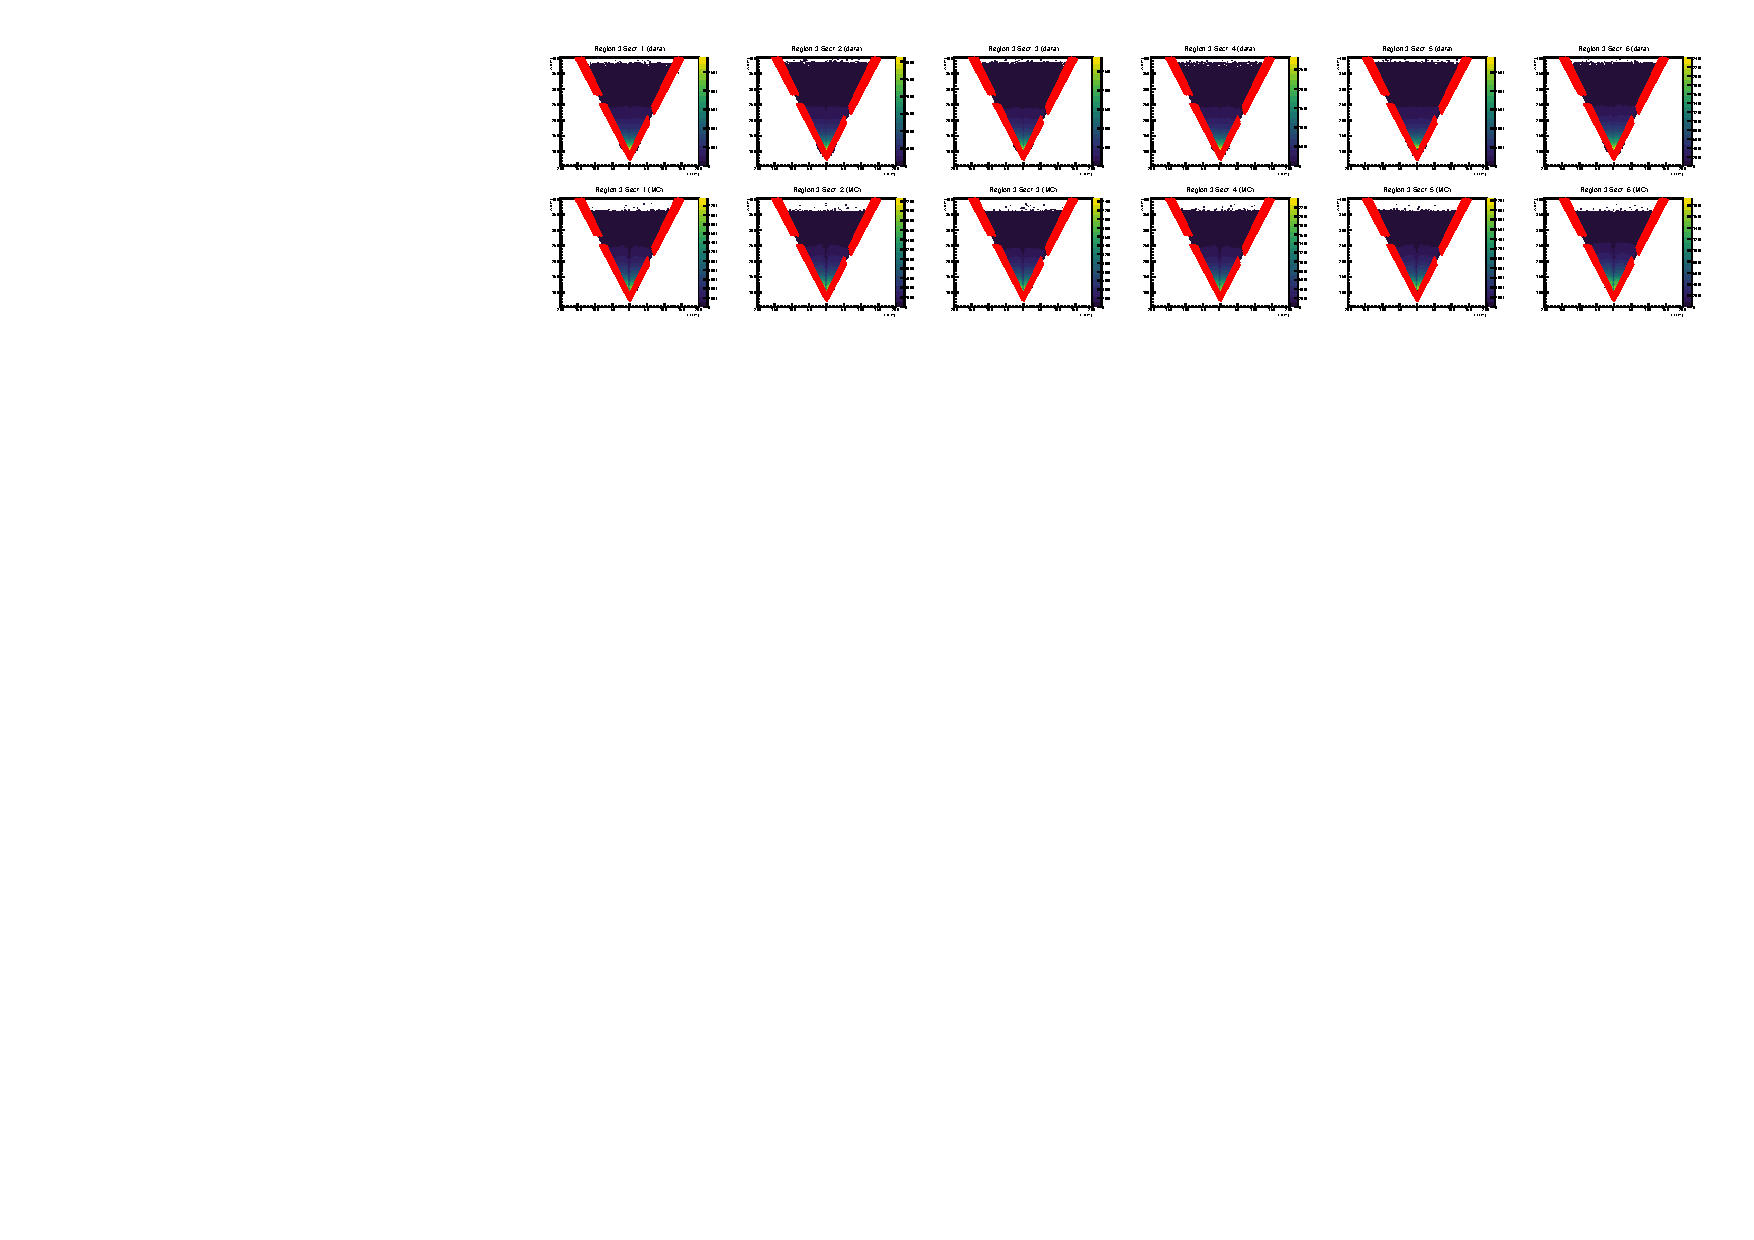
\includegraphics[width=\textwidth]{image/plots/sidis/systematics/region3.pdf}
  \caption[Systematic boundaries on region 3]{Boundaries for electron identification cuts placed on the region 3 drift chambers are shown for data (top row) and Monte Carlo (bottom row).}
\end{sidewaysfigure}

\begin{sidewaysfigure}
  \centering
  \label{fig:systematics-sampling-fraction}
  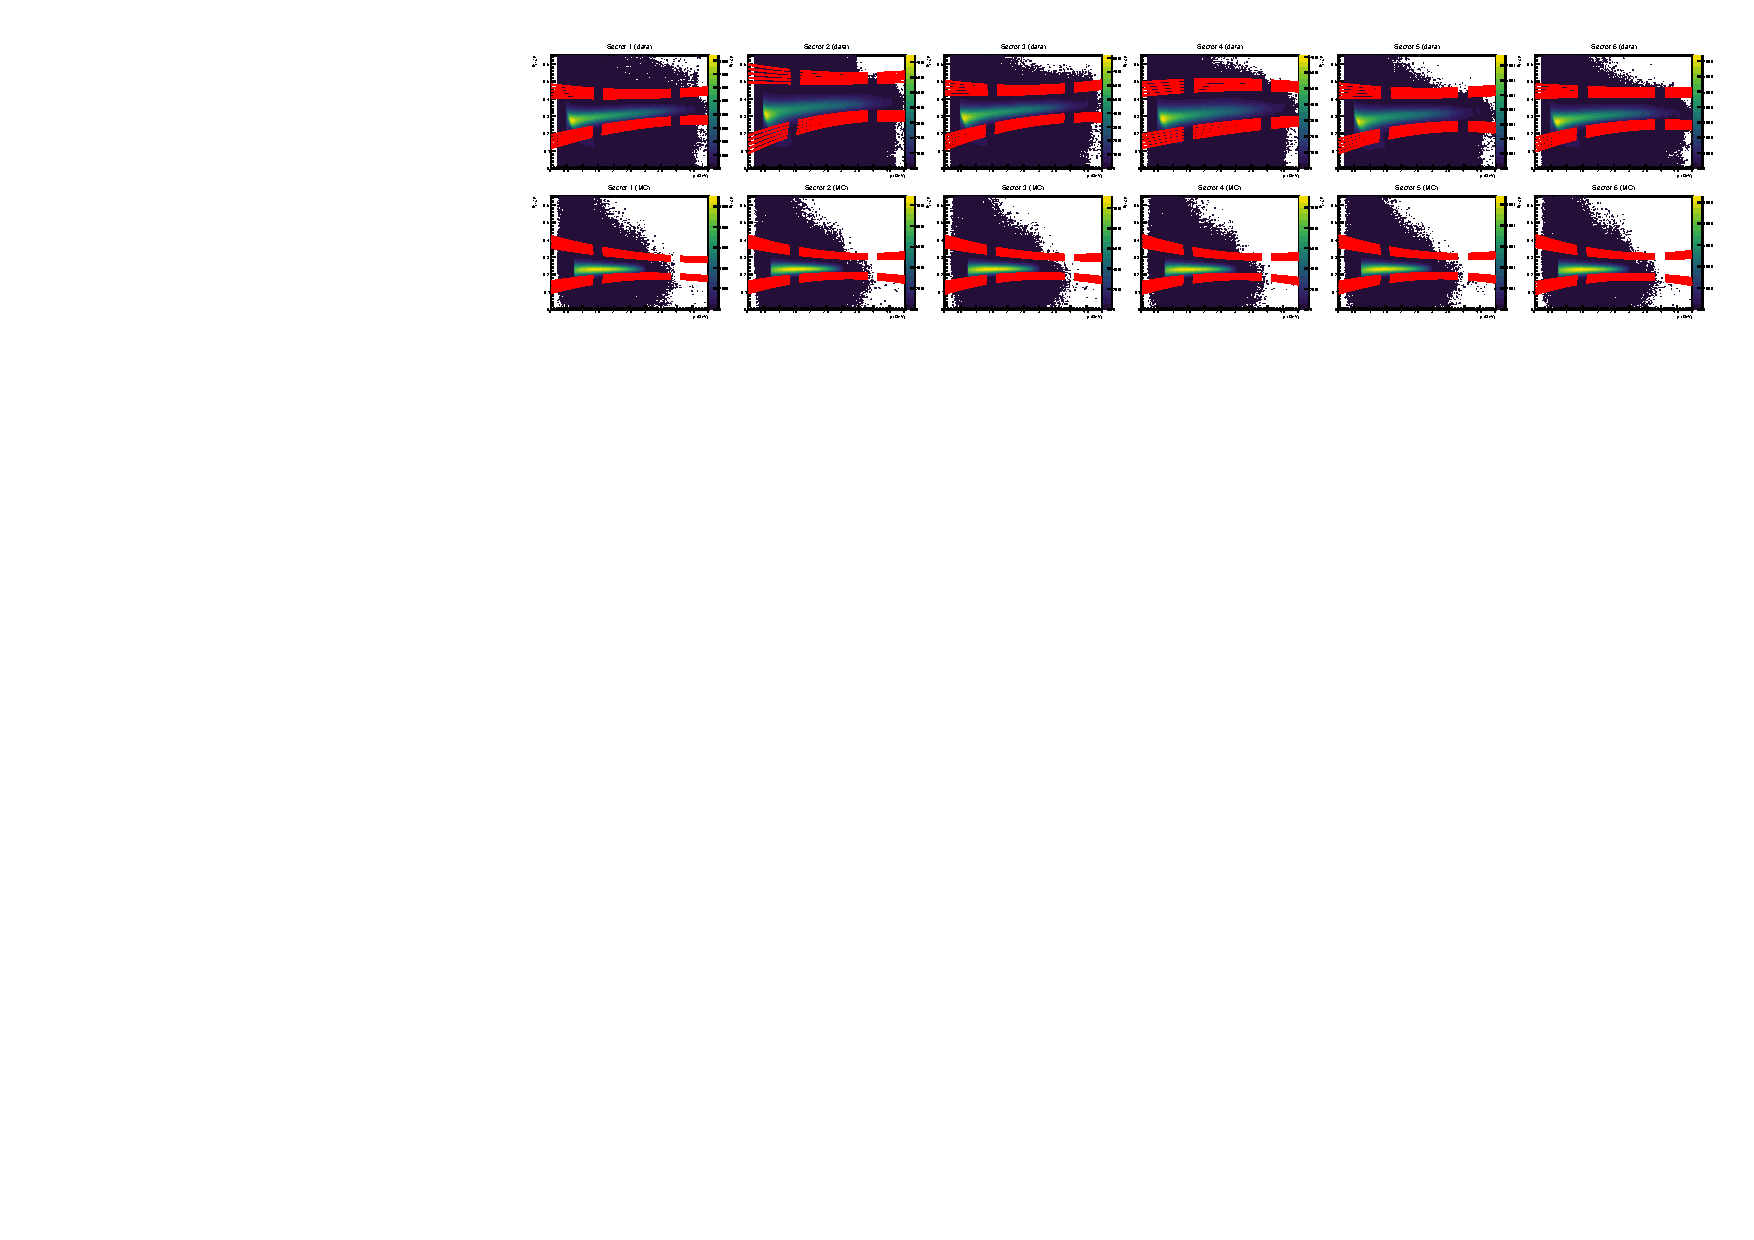
\includegraphics[width=\textwidth]{image/plots/sidis/systematics/sampling_fraction.pdf}
  \caption[Systematic boundaries on sampling fraction]{The sampling fraction boundaries used to identify electrons in data (top) and Monte Carlo (bottom) are shown over the distributions.}
\end{sidewaysfigure}

\begin{figure}
  \centering
  \label{fig:systematics-z-vertex}
  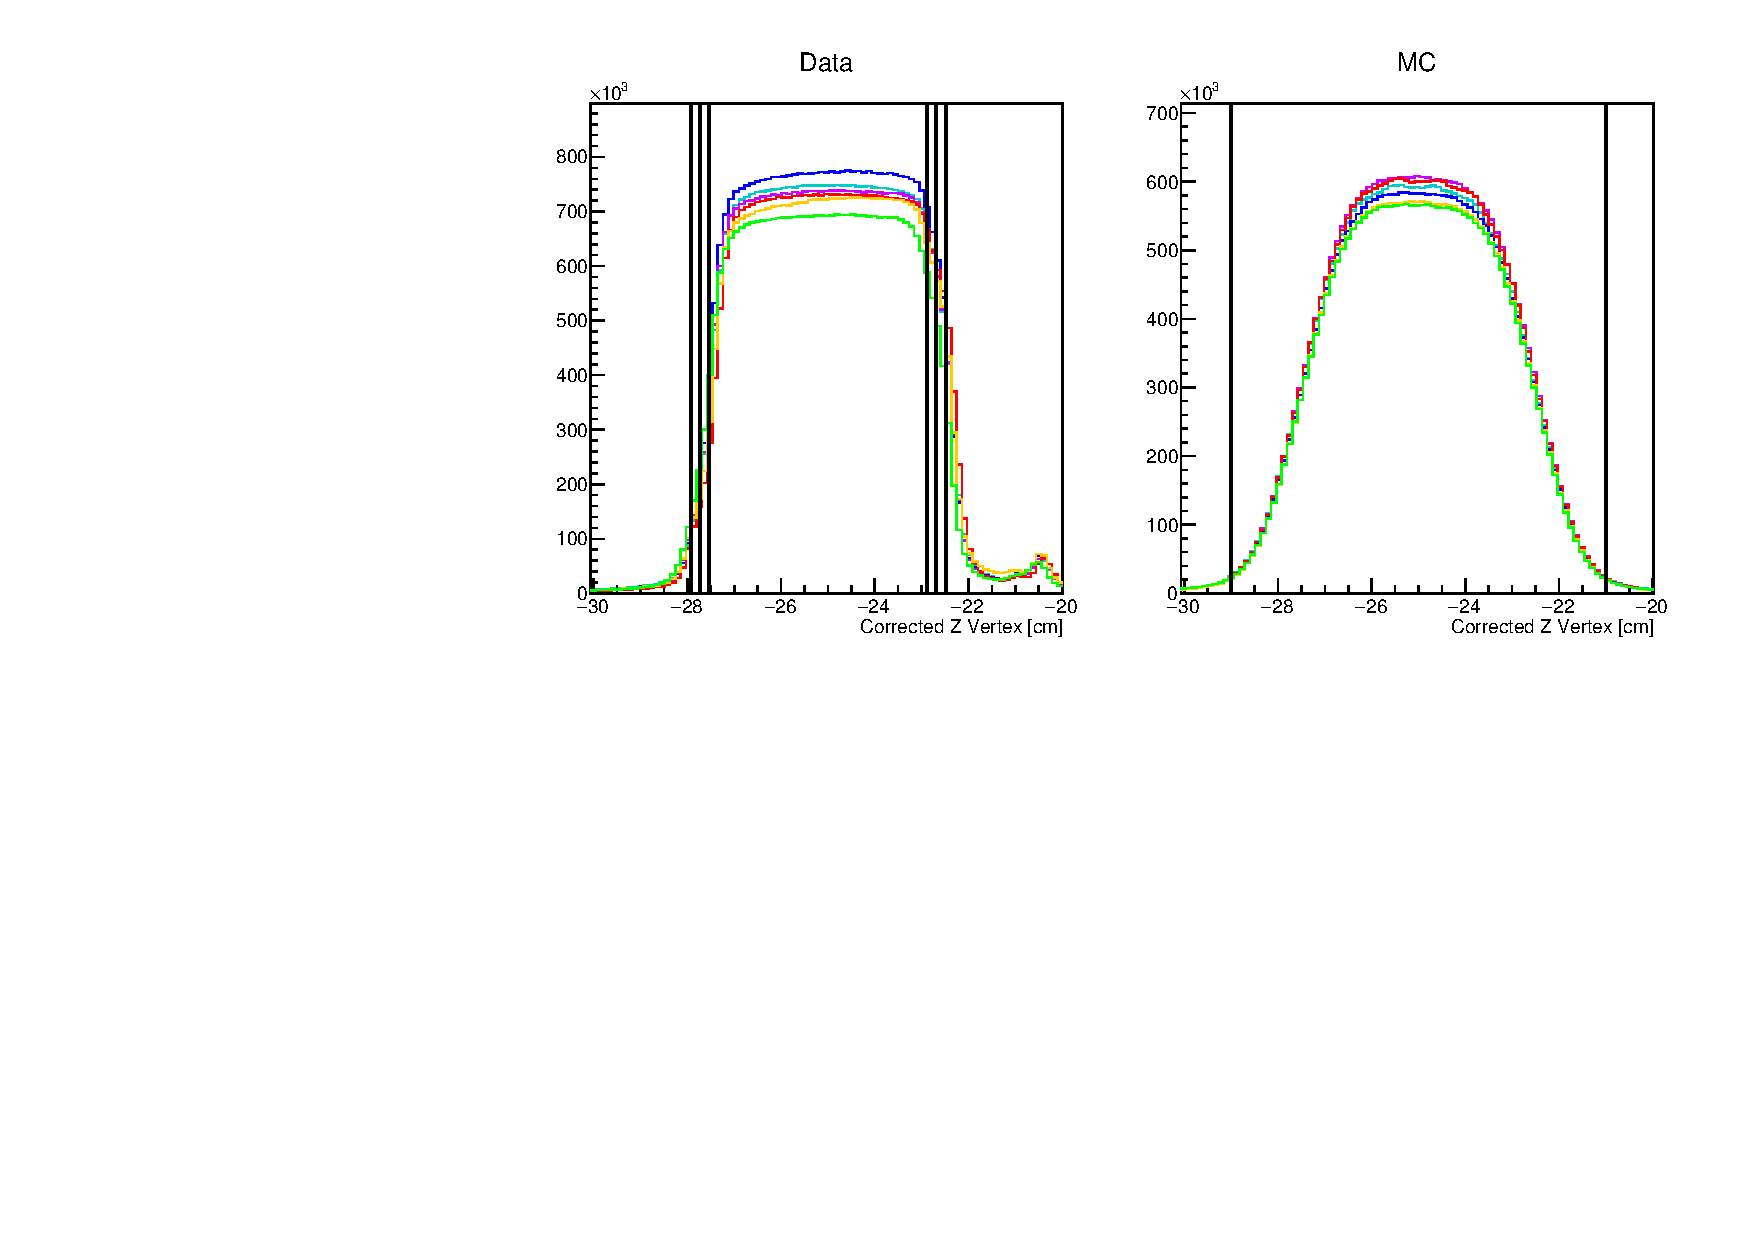
\includegraphics[width=\textwidth]{image/plots/sidis/systematics/z_vertex.pdf}
  \caption[Systematic variations of electron z-vertex cuts.]{The cut boundaries for z-vertex used to identify electrons in data (left) and Monte Carlo (right).  This histograms shown for data have been corrected before being filled.}
\end{figure}

\begin{figure}
  \centering
  \label{fig:systematics-ec-fid}
  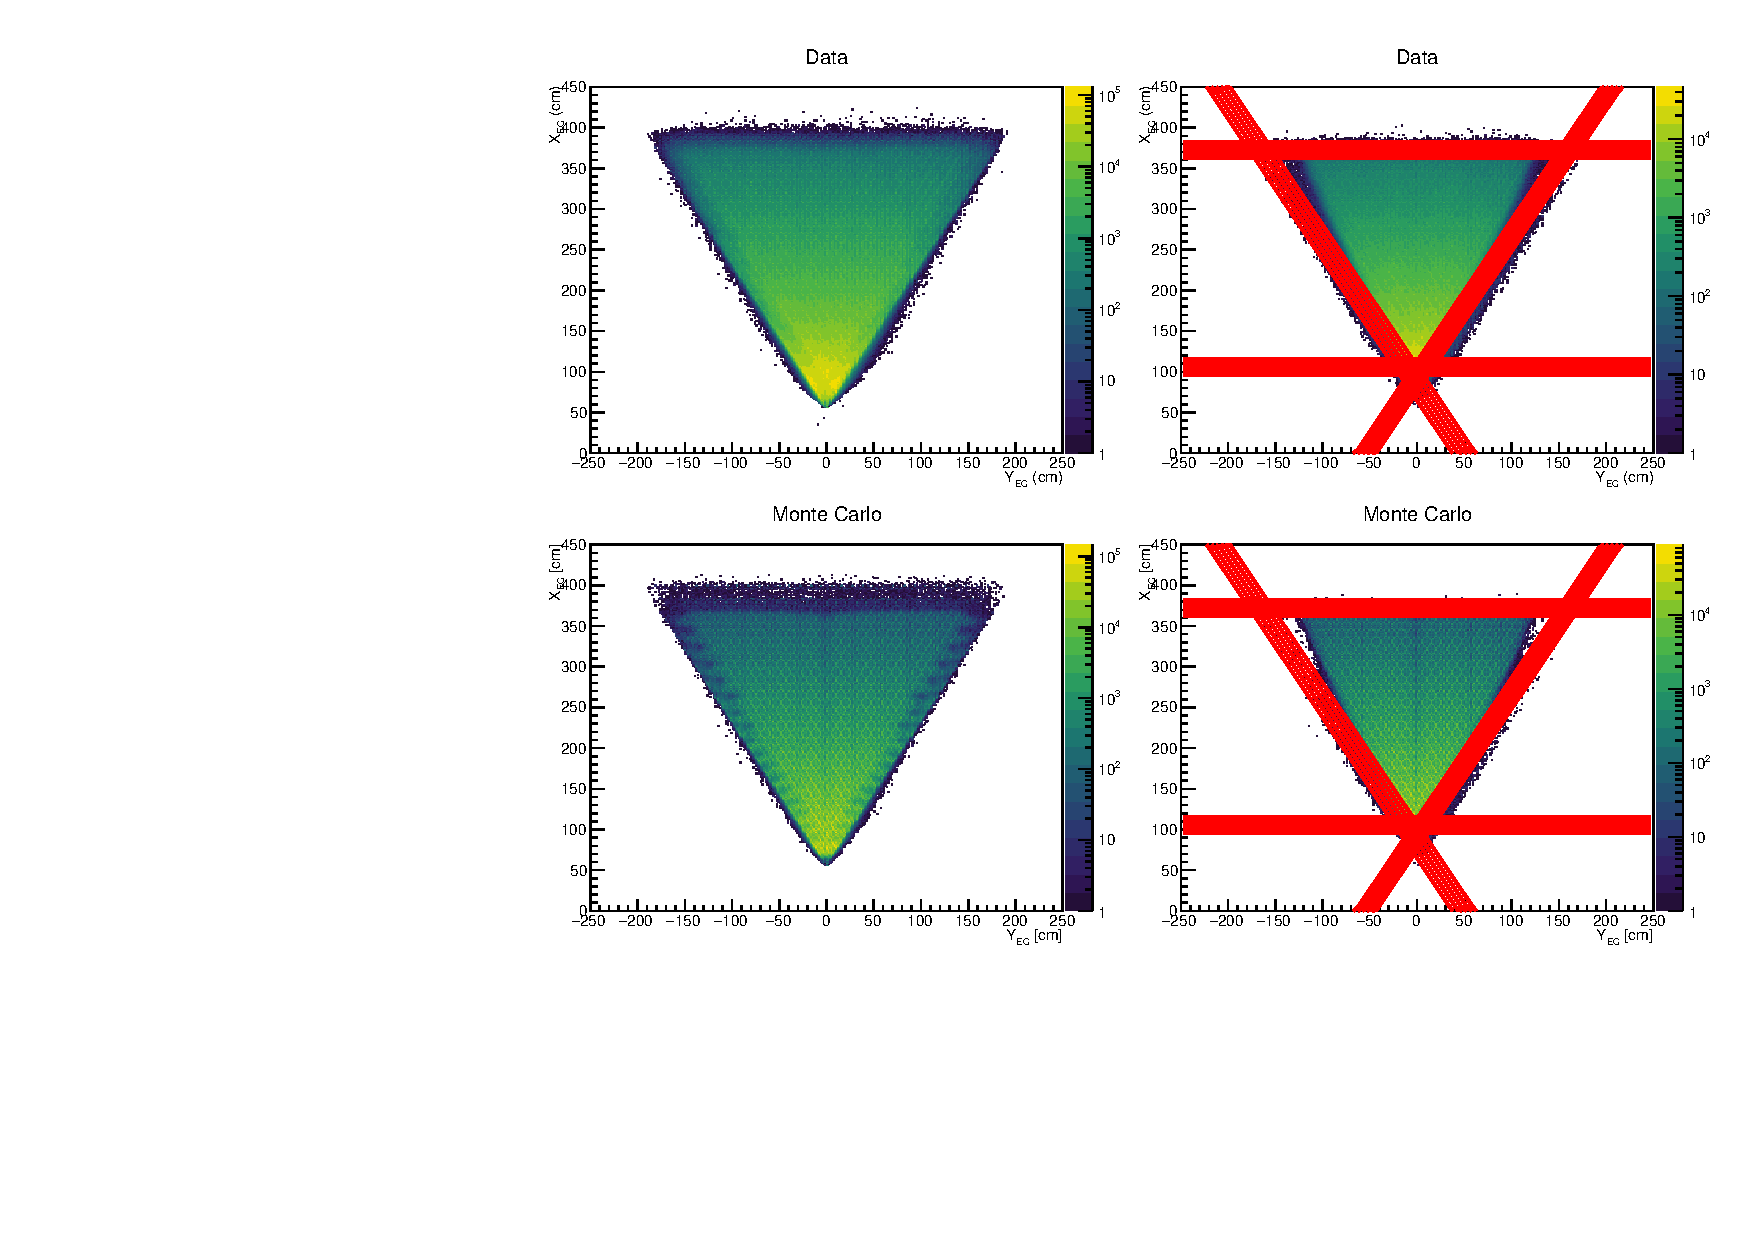
\includegraphics[width=\textwidth]{image/plots/sidis/systematics/ec_fid_sect1.pdf}
  \caption[Variation of EC U, V, and W cuts used to identify electrons.]{Electron identification cuts on U, V, and W coordinates are shown in x-y space.}
\end{figure}

\section{Results}
The big glorious conclusion of this study.